\documentclass[12pt]{article}
%\usepackage{makeidx}
%\usepackage{multirow}
%\usepackage{multicol}
%\usepackage[dvipsnames,svgnames,table]{xcolor}
%\usepackage{graphicx}
%\usepackage{epstopdf}
%\usepackage{ulem}
%\usepackage{amsmath}
%\usepackage{amssymb}

\usepackage[sorting=none]{biblatex}
\usepackage[french]{babel}
\usepackage{caption}
\usepackage{hyperref}
\usepackage[T1]{fontenc}
\usepackage{float}
\usepackage{graphicx}
\usepackage[utf8]{inputenc} 
\usepackage{csquotes}
\usepackage{pdfpages}
\usepackage{url}

\addbibresource{webographie.bib}

\title{Rapport de stage}
\usepackage[paperwidth=595pt,paperheight=841pt,top=56pt,right=56pt,bottom=56pt,left=56pt]{geometry}

\makeatletter
	\newenvironment{indentation}[3]%
	{\par\setlength{\parindent}{#3}
	\setlength{\leftmargin}{#1}       \setlength{\rightmargin}{#2}%
	\advance\linewidth -\leftmargin       \advance\linewidth -\rightmargin%
	\advance\@totalleftmargin\leftmargin  \@setpar{{\@@par}}%
	\parshape 1\@totalleftmargin \linewidth\ignorespaces}{\par}%
\makeatother 

% new LaTeX commands
\parindent=5pt

\begin{document}


\begin{center}

\vspace{3pt} \noindent
\begin{tabular}{p{439pt}}
\parbox{439pt}{\centering 
\includegraphics[width=125pt]{gallery/img-3.png}\textbf{{\large 

\includegraphics[width=146pt]{gallery/img-2.png}
}}
\includegraphics[width=132pt]{gallery/img-1.png}{\small  }} \\

\hline
\vspace{5cm}
\parbox{439pt}{\centering 
{\Huge Rapport de stage TELECOM Nancy 2$^{e}$ année}
} \\
\vspace{1pt}
\parbox{439pt}{\centering 
\textit{{\Huge Editeur collaboratif pair-à-pair MUTE : Edition de texte riche}}
} \\
\vspace{2cm}
\parbox{439pt}{\centering 
\textbf{\textit{{\Large Camille Menou}}}
} \\
\parbox{439pt}{\centering } \\
\end{tabular}

\end{center}



\begin{center}
\textbf{Ann\'{e}e 2016-2017}
\end{center}

\begin{center}
Stage de 2$^{e}$ année réalisé dans l'équipe \textit{COAST}
\end{center}

\begin{center}
\begin{figure}[h]
  \begin{minipage}[c]{.46\linewidth}
    \centering
    
\includegraphics[scale=0.3]{gallery/loria.jpg}
  \end{minipage}
  \hfill
  \begin{minipage}[c]{.46\linewidth}
    \centering
    
\includegraphics[scale=0.20]{gallery/inria.png}
  \end{minipage}
\end{figure}
\end{center}

\vspace{3cm}
{\raggedright
Maître de stage~: \textit{Philippe Kalitine}
\\
Encadrant universitaire~: \textit{Alexandre Parodi}\pagebreak{}
}

\begin{center}
\textbf{{\huge Déclaration sur l'honneur de non-plagiat}}
\thispagestyle{empty}
\end{center}

\textbf{Je soussignée,}

Menou Camille

\textbf{\'{E}lève-ingénieure régulièrement inscrite en 2$^{e}$
année à TELECOM Nancy}

\textbf{N$^\circ{}$ de carte d'étudiant(e)~:} 13538235

\textbf{Année universitaire~:} 2016 - 2017

\textbf{Auteur(e) du document, m\'{e}moire, rapport ou code informatique
intitul\'{e}~:} Editeur collaboratif pair-à-pair MUTE : Edition de texte riche



Par la présente, je déclare m'être informée sur les
différentes formes de plagiat existantes et sur les techniques et normes de
citation et référence.

Je déclare en outre que le travail rendu est un travail original, issu de ma
réflexion personnelle, et qu'il a été rédigé entièrement
par mes soins. J'affirme n'avoir ni contrefait, ni falsifié, ni copié
tout ou partie de l'\oe{}uvre d'autrui, en particulier texte ou code
informatique, dans le but de me l'accaparer.

Je certifie donc que toutes formulations, idées, recherches, raisonnements,
analyses, programmes, schémas ou autre créations, figurant dans le
document et empruntés à un tiers, sont clairement signalés comme
tels, selon les usages en vigueur.

Je suis consciente que le fait de ne pas citer une source ou de ne pas la
citer clairement et complètement est constitutif de plagiat, que le plagiat est
considéré comme une faute grave au sein de l'Université, et qu'en cas
de manquement aux règles en la matière, j'encourrais des poursuites non
seulement devant la commission de discipline de l'établissement mais
également devant les tribunaux de la République Française.

\begin{center}
\textbf{Fait à Villers-lès-Nancy, le 24/08/2017}
\end{center}
\thispagestyle{empty}

\begin{center}
\textbf{Signature~:}
\end{center}

\newpage
\thispagestyle{empty}
\section*{Résumé :}
MUTE est un éditeur de texte collaboratif temps-réel pair-à-pair. Basé sur le framework Angular, il s'agit d'une interface développée par l'équipe COAST, au sein du LORIA. En vue d'une utilisation prochaine au sein de l'INRIA, cet éditeur open-source a été rendu riche en ajoutant des fonctionnalités autour de l'ajout de style, de formules mathématiques et de listes. Ce travail est basé sur de l'interopérabilité de solutions open-source et sur des directives visant à améliorer l'interface et l'expérience utilisateur.

\section*{Abstract :}
MUTE is a peer-to-peer collaborative real-time text editor. Based on Angular framework, it is developped by COAST team, in LORIA. For its usage inside INRIA, this open-source editor got rich by adding functionnalities around the addition of style, math formulas and lists. This work is based on interoperability of open-source solutions and on guidelines meant to improve the interface and the experience of the user.


%Pour insérer une image facilement :
%\begin{figure}[H]
%\centering
%\includegraphics[scale=0.4]{fichier de l'image}
%\caption[nom dans le sommaire]{légende}
%\label{fig:gallery}
%\end{figure}

\newpage
\thispagestyle{empty}
\section*{Remerciements}
Mes tout premiers remerciements sont adressés à M. Philippe Kalitine, ingénieur de recherche chez COAST et mon maître de stage. Merci pour la confiance, l'indépendance et l'expertise qui m'ont permises de mener à bien les tâches qui m'étaient confiées.\\

Merci à TELECOM Nancy pour la mise en place de cette période de stage afin que ses étudiants de seconde année puissent acquérir une expérience technique indispensable à la formation d'un ingénieur.\\

Merci à mon encadrant universitaire, M. Alexandre Parodi pour la supervision de ce stage et la lecture et notation de ce rapport.\\

De manière générale merci à toute l'équipe COAST pour sa convivialité. Venir travailler avec vous ce n'était plus du travail, mais l'exercice d'une passion commune dans une excellente ambiance !\\

Enfin, je tiens à remercier toutes les personnes qui se sont donnés la peine de relire ce rapport : M. Philippe Kalitine, M. Matthieu Nicolas et M. Gwendal Le Fur.

\newpage
\thispagestyle{empty}
\tableofcontents

\newpage
\setcounter{page}{1}
\addcontentsline{toc}{section}{Introduction}
\section*{Introduction}
\paragraph{}
Dans le cadre de ma deuxième année dans l'école d'ingénieur TELECOM Nancy, j'ai effectué un stage technicien au Laboratoire lorrain de recherche en informatique et ses applications (LORIA) \cite{loria} à Vand\oe{}uvre-lès-Nancy. Durant dix semaines j'ai travaillé au sein de l'équipe COAST \cite{coast} dirigée par François Charoy, du 6 juin au 11 août de l'année 2017. Ce stage m'a été proposé par Philippe Kalitine, ingénieur en recherche en informatique chez COAST.

\paragraph{}
L'équipe travaille actuellement sur MUTE \cite{mute}, un éditeur web de texte collaboratif pair-à-pair open source. Il s'agit d'une application semblable à Google Doc qui ne nécessite pas l'utilisation d'un serveur pour fonctionner. A terme, MUTE a pour vocation de devenir l'éditeur de texte principal du personnel Inria \cite{inria}.

\paragraph{}
L'objectif de mon stage était de rendre l'éditeur riche, par exemple en intégrant des fonctionnalités autour de l'ajout de style dans les documents, d'images, de formules mathématiques, ou bien autour de l'exportation dans divers formats (PDF, HTML, etc.).

\paragraph{}
Dans le contexte de ce stage qui est celui de la recherche, le mode de travail ainsi que les enjeux sont différents du monde de l'entreprise. S'il n'y a pas un client à qui l'on doit livrer l'application, l'équipe COAST est néanmoins soumise à une deadline. En effet, l'équipe se prépare à faire une démonstration de MUTE lors de la quinzième European Conference on Computer-Supported Cooperative Work (ECSCW) \cite{ecscw} et qui aura lieu du 28 août au 1er septembre 2017 à Sheffield (UK). L'enjeu n'était donc pas des moindres et nécessitait un travail de qualité.

\paragraph{}
Ce document constitue le rapport de ce stage. Dans un premier temps, nous poserons le contexte en parlant de l'équipe COAST au sein du LORIA et de ses axes de recherche. S'ensuivront une mise en lumière de l'origine du projet ainsi que les objectifs du stage. Nous détaillerons ensuite l'ensemble des travaux réalisés, les résultats obtenus et les difficultés rencontrées. Enfin, nous dresserons un bilan de cette expérience technique en laboratoire de recherche et parlerons d'éventuelles améliorations à apporter au projet.\\

\newpage
\section{L'équipe COAST : présentation}
\subsection{LORIA}
\paragraph{}
Le LORIA est une Unité Mixte de Recherche (UMR) \cite{umr} composée du Centre National de la Recherche Scientifique (CNRS) \cite{cnrs}, de l'Université de Lorraine \cite{univ}, et Inria. Créé en 1997, le LORIA est investi dans la recherche fondamentale et appliquée en sciences informatiques. Le LORIA fait aussi partie de la Fédération Charles Hermite \cite{hermite} et du pôle scientifique Automatique, Mathématiques, Informatique et leurs interactions (AM2I) \cite{am2i} de l'Université de Lorraine.
\paragraph{}
D'après son site Internet, en août 2017, ce ne sont pas moins de ving-neuf équipes, soit plus de quatre cents personnes qui travaillent au Loria. Les équipes sont réparties dans cinq départements :
\begin{itemize}
    \item Département 1 : Algorithmique, calcul, image et géométrie
    \item Département 2 : Méthodes formelles
    \item Département 3 : Réseaux, systèmes et services
    \item Département 4 : Traitement automatique des langues et des connaissances
    \item Département 5 : Systèmes complexes, intelligence artificielle et robotique
\end{itemize}
On retrouve ces départements dans l'organigramme ci-après, extrait du site du LORIA. 

\paragraph{}
Le conseil scientifique est composé du directeur, des deux directeurs adjoints et des responsables des cinq départements décrits plus haut. Tous les quinze jours, ils se réunissent afin d'assister le directeur dans les décisions concernant le LORIA.
\paragraph{}
Le conseil de laboratoire est composé de représentants de l'ensemble du personnel du LORIA. Tous les deux mois, il permet de débattre sur des questions de  politique scientifique, organisation du laboratoire, budget, recrutement de personnels, formation, règlement intérieur, aménagement du temps de travail, conditions de travail et consultation des personnels...

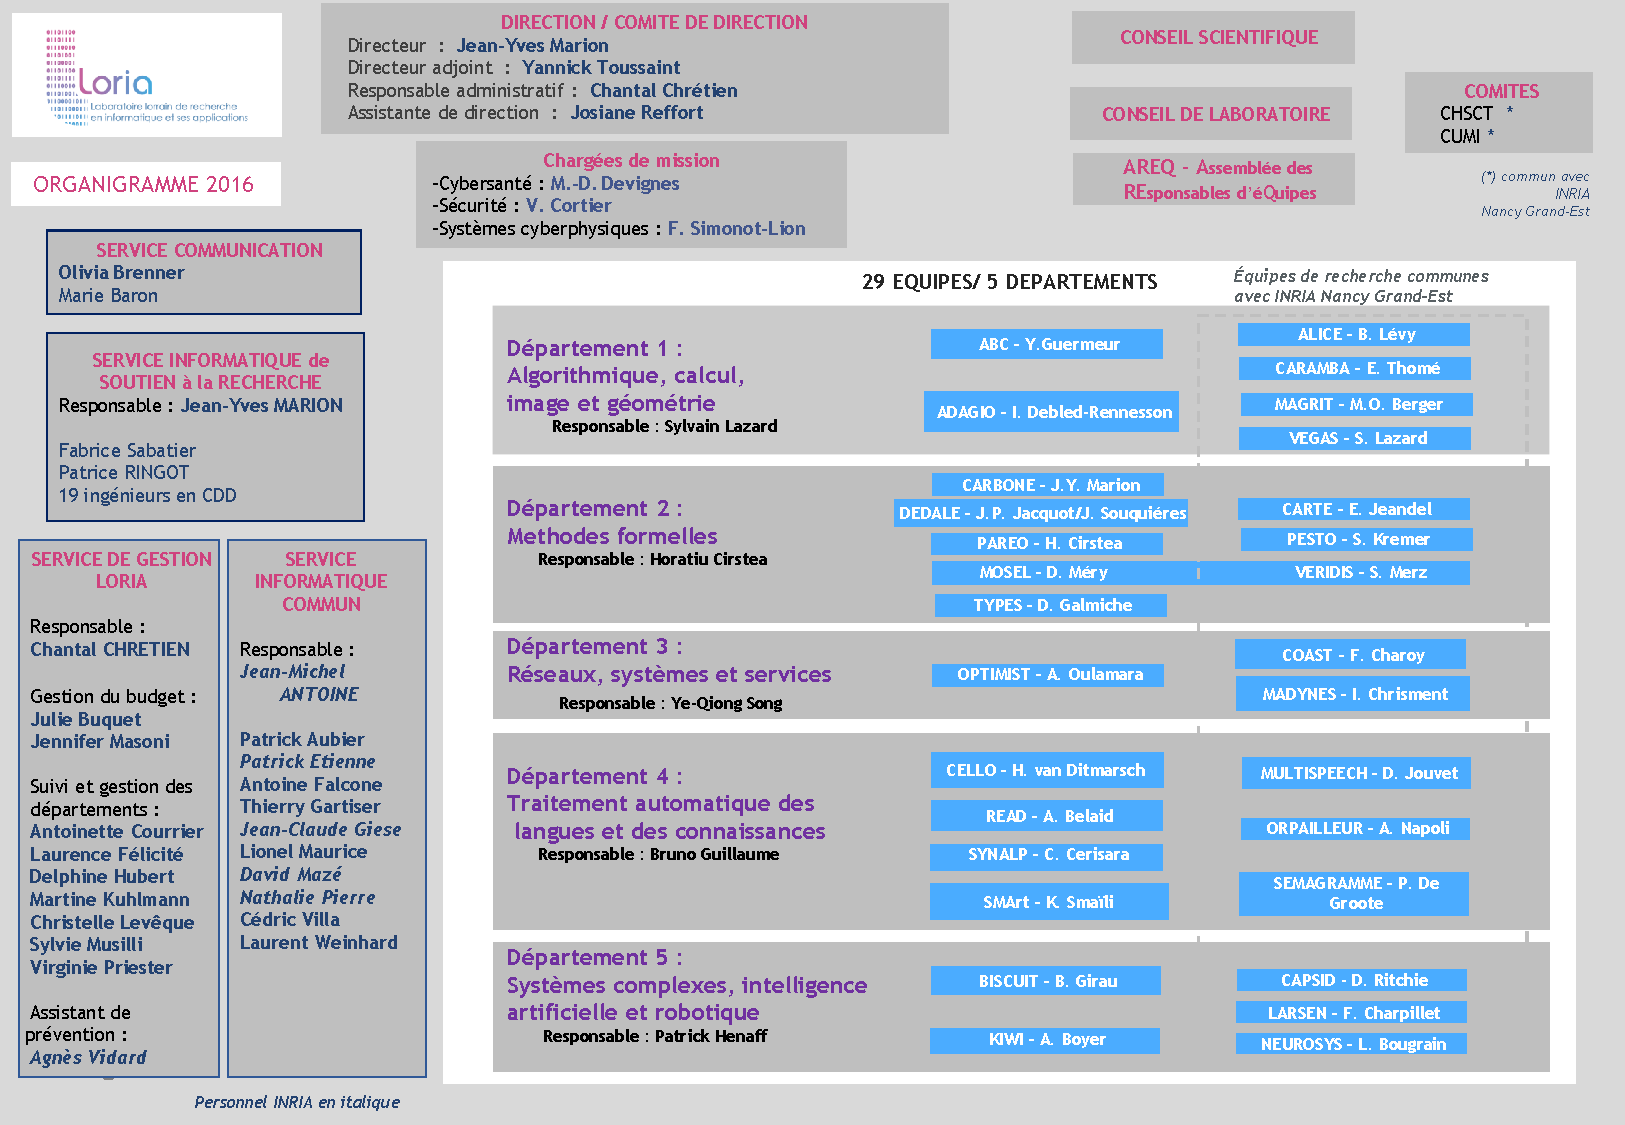
\includepdf[pages={1},landscape=true]{gallery/organigrammeLORIA.pdf}

\subsection{L'équipe COAST}
\paragraph{}
Comme on peut le constater sur l'organigramme du LORIA, l'équipe COAST, dirigée par M. François Charoy, se trouve dans le département associé aux Réseaux, systèmes et services. L'équipe travaille effectivement dans ce domaine mais également dans le calcul distribué. Ses thématiques de recherche sont les systèmes distribués et intergiciels \footnote{Aussi appelé "middleware", un intergiciel est un logiciel tiers qui crée un réseau d'échange d'informations entre différentes applications informatiques}.
\paragraph{}
Le projet de cette équipe est \emph{"de définir des méthodes et des techniques permettant la construction d'applications collaboratives de confiance, basée sur une connaissance précise des algorithmes de réplication, sur la composition sure de service et sur une qualité de service qui peut être déduite et mesurée. Dans ce nouveau contexte, il est difficile de fournir des garanties prouvées sur les services. [Ils proposent] de baser [leur] travail sur une approche contractuelle et mesurable pour donner aux utilisateurs confiance dans les services qu'ils utilisent.  
Les axes de recherche de l'équipe COAST sont les suivants :}
\begin{itemize}
  \item \emph{La gestion sure et efficace de données collaborative à large échelle en terme de quantité de données et d'utilisateurs de ces données.}
  \item \emph{La composition de services orientés données pour permettre la construction d'applications à l'échelle du Web et pour donner des garanties sur le fonctionnement de ces applications.}
  \item \emph{Le support à la construction d'environnements collaboratifs pour lesquels on puisse déterminer un niveau de confiance et de sécurité" \footnote{Sources : \href{https://www.inria.fr/equipes/coast}{https://www.inria.fr/equipes/coast}}.}
\end{itemize}

\paragraph{}
L'équipe COAST est composée d'une chercheuse scientifique, de dix membres de facultés (professeurs ou assistants professeurs), de trois ingénieurs de recherche (dont mon maître de stage), de dix étudiants en thèse, de deux post-doctorants et de trois assistantes administratives. Pendant cette période de stage, nous étions également trois stagiaires de la promotion vingt-six de TELECOM Nancy. En Figure \ref{orga}, un organigramme de l'équipe COAST.

\newpage
\begin{figure}[H]
    \centering
    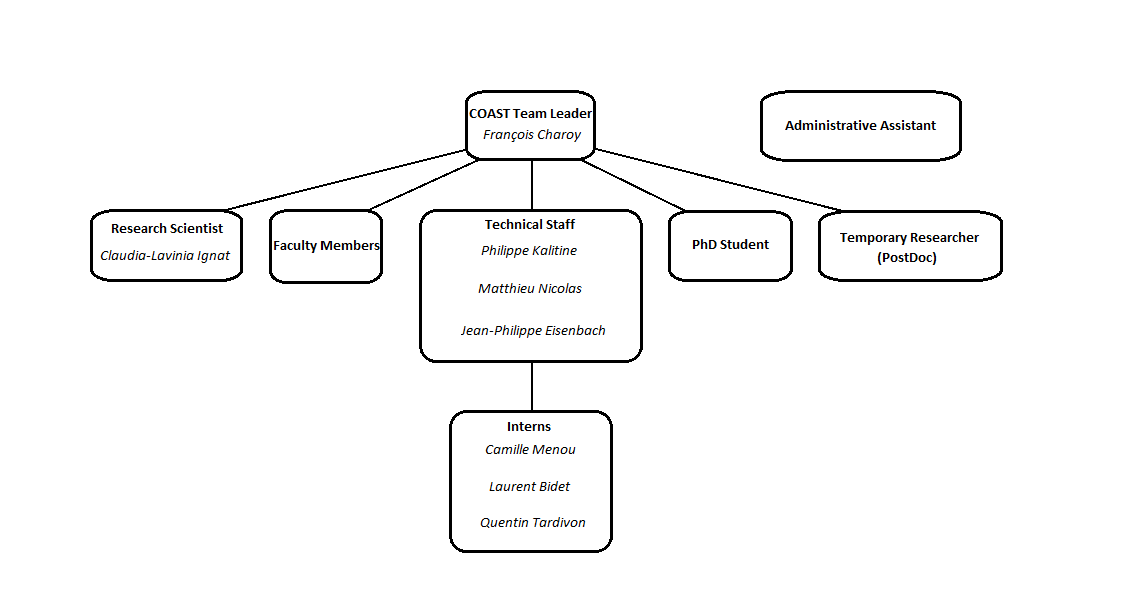
\includegraphics[scale=0.85, angle=90]{gallery/organigrammeCOAST.png}
    \caption[nom dans le sommaire]{Organigramme équipe COAST}
    \label{orga}
\end{figure}

\newpage
\section{Problématique du stage : rendre un éditeur de texte riche}
\subsection{Mise en contexte : MUTE}
\paragraph{Origine du besoin}
A l'heure actuelle, au sein des entreprises, l'édition et le partage de fichiers entre collègues se fait très souvent sous forme de mail où le fichier est mis en pièce jointe. Cette pratique est très contraignante pour plusieurs raisons :\\
\begin{itemize}
    \item c'est une procédure chronophage.
    \item les modifications apportées ne sont pas évidentes à voir.
    \item si beaucoup de personnes doivent modifier le même document et plus précisément un même paragraphe, la fusion de ces modifications devient très laborieuse.
    \item l'envoi d'un mail contenant des rapports confidentiels expose l'entreprise à des espionnages industriels.
\end{itemize}
\paragraph{}
Pour pallier ce problème, certains proposeraient tout simplement d'utiliser Google Doc, l'éditeur de texte de Google, qui a l'avantage d'apporter une édition collaborative d'un document et en temps-réel. Malheureusement, Google Doc utilise une architecture dite, centralisée : un serveur stocke le document et écoute les modifications des collaborateurs. De cela découlent trois inconvénients majeurs empêchant la mise en place de cette solution en entreprise :\\
\begin{itemize}
    \item l'utilisation de l'éditeur ne passe pas à l'échelle.
    \item le fait que le document soit stocké sur les serveurs de Google ne plaît pas aux entreprises pour une question de sécurité (vol de données) mais aussi de sûreté (la sauvegarde du document peut être compromise si les serveurs de Google subissent une panne).
    \item l'édition d'un document devient impossible si les serveurs de Google sont en difficulté ou si notre connexion internet devient instable.
\end{itemize}
\paragraph{}
Afin de développer une plate-forme collaborative permettant de répondre à ces besoins, le projet OpenPaaS::NG \cite{openpaas} a été créé. Financé par BpiFrance \cite{bpi}, ce projet open-source français est réalisé en collaboration avec les sociétés Linagora \cite{linagora}, XWiki SAS \cite{xwiki}, Nexedi \cite{nexedi} et le laboratoire d'informatique de l'école polytechnique.
\paragraph{}
A cette intention, l'expertise de l'équipe COAST a été requise. Leur rôle a été de montrer qu'il est possible de mettre en place
\begin{itemize}
    \item un réseau pair-à-pair capable de mieux passer à l'échelle que Google Doc.
    \item une collaboration sûre (sans pertes de données).
\end{itemize}
\paragraph{}
COAST a donc créé l'API indépendante mute-core \cite{mute-core}, constituée de deux sous-projets :

\paragraph{Mute-structs}
Mute-structs \cite{mute-structs} est un projet Node.js qui propose une implémentation de l'algorithme CRDT (Conflict-free replicated data type) LogootSplit \cite{logoot}. Cet algorithme est issu d'une thèse provenant de l'équipe COAST et sert à la fusion des contributions des collaborateurs sans générer de doublons ou de perte de données.

\paragraph{Netflux}
Nextflux \cite{netflux} est une API permettant l'établissement d'un réseau pair-à-pair.

\paragraph{MUTE}
Les ingénieurs de l'équipe développent l'application MUTE qui met donc en valeur ces résultats de recherche. Multi User Text Editor (MUTE) est donc une interface web basée sur l'API CodeMirror et qui se sert de l'API mute-core. MUTE est donc un éditeur web collaboratif temps-réel pair-à-pair.
\paragraph{}
Si MUTE n'avait au début vocation qu'à ne servir que de plateforme de démonstration pour Netflux et mute-structs, MUTE doit maintenant devenir utilisable au sein de l'INRIA.

\subsection{Description et analyse du problème posé : apporter une édition riche}
\paragraph{}
Afin de rendre l'éditeur utilisable au sein d'INRIA, il est nécessaire de le rendre riche. Il s'agissait donc d'ajouter des nouvelles fonctionnalités autour de l'édition pour améliorer l'expérience utilisateur.
\paragraph{}
Il fallait pouvoir ajouter du style au texte (gras, italique...), des gestions de listes, des liens hypertextes, des images ou des formules mathématiques. Il fallait proposer plusieurs manières d'ajouter ce style : écriture de la syntaxe nécessaire à la main, à l'aide de raccourcis clavier, ou grâce à des éléments visuels cliquables.
\paragraph{}
Ces manières d'ajouter doivent être simples d'utilisation, intuitives et rester dans la norme de ce qui existe en termes d'édition, de traitement de texte, afin de ne pas perturber l'expérience utilisateur.
\paragraph{}
De plus, étant donné que LogootSplit ne traite que du texte brut, il est nécessaire que les solutions apportées ne nécessitent pas un transfert d'informations aux collaborateurs par un moyen autre que du texte.

\subsection{Cahier des charges}
Le cahier des charges du projet a été défini comme étant les tâches GitHub (plus communément appelées par le terme anglais "issues") auxquelles j'étais assignée. Les détails nécessaires m'ont été fournis à l'oral au moment opportun. De part le caractère open-source du projet, le cahier des charges a été rédigé en anglais.
Avant de passer à la lecture du cahier des charges, il est nécessaire d'expliquer ce qu'est Markdown. Markdown est un langage de balisage qui permet d'ajouter du style au texte (gras, italique, listes, liens, titres...). Un langage de balisage est un langage de description de données utilisant des balises. Soit la syntaxe **exemple**. Les astérisques sont les balises, "exemple" la donnée à décrire. En Markdown, cette syntaxe signifie que la donnée "exemple" doit être mise en gras.
Ci-dessous, la liste des issues que je devais réaliser pendant mon stage :\\

As a User I want to :
\begin{description}
    \item [see a partially styled (inline rendered style) Markdown text in the editor :] les balises correspondant à de la syntaxe Markdown doivent être camouflées après interprétation, une fois que l'édition du texte stylisé est terminée ou qu'on clique sur un autre élément que celui-ci. De même, les balises doivent réapparaître lorsque l'utilisateur met le focus sur un élément contenant du style.
    Plus précisément, quand on écrit **exemple**, tant que le curseur se trouve dans ce texte, on doit voir les balises. Mais quand le curseur n'est plus sur cette zone, on ne doit voir que "exemple", en gras.
    \item [see a rendered version of my document :]MUTE aurait dû être divisée en deux parties : à gauche l'utilisateur écrirait le texte souhaité, à droite il aurait accès à un rendu où la syntaxe aurait été interprétée. Cette issue est devenue obsolète du fait de la précédente (voir explications dans la partie Réalisation et validation). Si l'issue précédente n'était pas réalisable immédiatement, il aurait fallu faire cette issue, étape intermédiaire entre ce qui existait au début du stage, et ce qui existe maintenant.
    \item [have an outline view for Markdown :] l'utilisateur doit pouvoir accéder à une table des matières du document à côté de ce dernier. Lors de la création d'un titre (balises \#, \#\#, etc...), le texte associé doit apparaître dans la table des matières. Lors du parcours du document, le titre correspondant à la partie actuellement visible du document doit être mis en valeur dans cette table (mis en gras par exemple).
    \item [add basic styles (bold, italic...) to the document using keyboard shortcuts :]l'utilisateur doit pouvoir ajouter/enlever du style en utilisant des raccourcis claviers intuitifs, par exemple Ctrl+B pour le gras.
    \item [add basic styles (bold, italic...) to the document using toolbar :]au moment d'une sélection de texte, une barre d'outils doit apparaître pour que l'utilisateur puisse ajouter/enlever le style à la souris.
    \item [see my math formula rendered :]l'utilisateur doit pouvoir écrire une formule mathématique et qu'elle ait le même rendu que s'il l'avait écrite à la main.
    \item [include images into my documents :]tout est dans l'intitulé.
    \item [to add some "End of Page" character :]au bout d'un certain nombre de lignes, la page doit se terminer et une nouvelle doit être créée.
    \item [consult Markdown cheat-sheet :]l'utilisateur doit pouvoir rapidement accéder à la syntaxe de Markdown
    \item [consult MathJax cheat-sheet :]l'utilisateur doit pouvoir rapidement accéder à la syntaxte de MathJax
    \item [be able to export the document to another document format (PDF, plain text) :]tout est dans l'intitulé.\\
\end{description}

Les issues à propos des cheat-sheets et de l'exportation comportaient le label \footnote{Aussi appelé 'tag', il s'agit d'un mot permettant de décrire ou de mettre une issue dans une catégorie. Par exemple le label 'bug' signifie que l'issue décrit le dysfonctionnement d'une fonctionnalité.} "optionnal" pour dénoter une priorité basse. Les autres issues ont été classées par ordre de priorité décroissante, comme ci-dessus.

L'ensemble de mon travail était régi par un besoin fonctionnel incontournable : si des fonctionnalités visent à modifier le contenu du document alors le contenu doit effectivement être modifié, et ce pour n'importe quel collaborateur du document. Un autre besoin, non négligeable, était que les développements marchent à la fois sur Chrome et sur Firefox.

\newpage
\section{Réalisation et validation}
\subsection{Auto-formation}
\paragraph{}
Le stage a d'abord commencé par une période d'auto-formation à base de Massive Open Online Courses (MOOCs), de vidéos de conférences et d'articles écrits par des développeurs/ingénieurs de la communauté informatique. A cette occasion, et pendant les onze premiers jours je me suis donc formée en JavaScript et en TypeScript (JavaScript typé).
\paragraph{}
Le projet utilisant le framework AngularJS j'ai également lu à ce sujet grâce à la Tour of Heroes \cite{tour}, projet Angular écrit pour un tutoriel disponible sur le site officiel d'Angular \cite{angular}.

\subsection{Environnement de travail}
\paragraph{}
La partie édition de MUTE est basée sur une API qui s'appelle CodeMirror \cite{codemirror}. Il s'agit d'un éditeur de texte écrit en JavaScript et pensé pour les navigateurs. Ce projet assez populaire (12,364 stars et 3000 forks au 4 août 2017) est agrémenté d'addons permettant d'étendre les fonctionnalités de CodeMirror au besoin.

\paragraph{}
L'ensemble du projet est hébergé sur un répertoire GitHub, un gestionnaire de version.

\paragraph{}
Il m'a été conseillé d'utiliser l'IDE (Integrated Development Environment) VisualStudio Code pour développer. Particulièrement adapté au langage JavaScript, VisualStudio permet de voir très facilement les fichiers modifiés par rapport au dernier commit et de faire des merges très simplement.

\paragraph{}
Le projet utilise le framework Angular. Ce framework est centré autour de la notion de composant. Un composant gère une partie de la vue (l'interface). Un composant est constitué :
\begin{itemize}
    \item d'un fichier JavaScript (en l'occurrence TypeScript) qui contient les données à afficher ainsi que les fonctions gérant leur comportement,
    \item d'un fichier HTML qui permet de structurer les données de l'interface,
    \item d'un fichier CSS qui contient les éléments de style à appliquer aux données.
\end{itemize}

\paragraph{}
Le projet utilise npm \cite{npm} afin de gérer ses dépendances.\\

\subsection{Méthode de travail}
Deux outils m'ont quotidiennement aidée à m'organiser et à prendre des notes pour faciliter l'écriture de ce rapport : l'outil de gestion de projet GitHub, ainsi qu'un journal quotidien que j'ai tenu selon le principe du bullet journal \cite{bullet}.

\paragraph{GitHub workboard}
Il s'agit d'un tableau référençant l'ensemble des issues m'étant attribués, de la documentation et ma roadmap. Une roadmap est le terme employé pour parler de l'organisation des issues dans le temps. L'organisation se fait de manière hebdomadaire. Vous trouverez un aperçu de ce tableau en Annexe A.
\paragraph{}
C'était un excellent moyen pour accéder rapidement à mes issues et cela permettait également à mon maître de stage de pouvoir jeter un oeil à mon avancement.\\

\paragraph{Journal quotidien}
Afin de noter un maximum de choses pour écrire ce rapport mais aussi pour noter ma réflexion, ne pas oublier de faire quelque chose ou juste mieux m'organiser, j'ai pris l'initiative de tenir un journal quotidien de mon travail. A cette occasion j'ai repris quelques principes des bullet journals comme par exemple le fait de noter systématiquement les tâches à faire en organisant des checklists. Pour lier le workboard au journal, j'ai noté chaque jour sur quelle(s) issue(s) j'ai travaillé avec un code couleur pour retrouver plus rapidement des notes que j'aurais prises à l'intention de l'une d'elles.\\

\paragraph{Compléter une issue}
Avant de commencer une issue, j'en informais mon maître de stage qui me donnait certaines pistes de réflexion et de recherche à explorer avant de commencer.
\paragraph{}
Ainsi, en toute autonomie, je menais des recherches les plus exhaustives possibles pour trouver des solutions open source ou juste des méthodes que j'aurais pu reproduire dans notre projet. Nous décidions ensuite ensemble du meilleur choix.
\paragraph{}
Après le développement de la solution, je présentais le résultat, relevant les limites et recevant des détails à rajouter au développement. Pour certaines issues, notamment pour les raccourcis clavier et la barre d'outils, je référençais sur l'issue correspondante l'ensemble des fonctionnalités présentes. En Annexe B, un exemple.
\paragraph{}
L'avantage de cette pratique est qu'il sera possible pour les personnes qui maintiendront mon code de voir s'il y a eu des régressions ou tout simplement de voir ce qui existe déjà et ce qu'il reste à faire.\\

\paragraph{Communication avec l'équipe}
Lors des premières semaines, chaque vendredi, l'équipe se réunissait pour faire état de l'avancement de chacun.
L'équipe utilise également Slack \cite{slack} pour communiquer.\\

\newpage
Abordons maintenant de manière plus concrète les différentes étapes de réalisation du cahier des charges.\\

\subsection{Cacher la syntaxe Markdown : intégration d'HyperMD}
Afin d'apporter du style à l'éditeur (gras, italique, etc.), l'équipe a décidé d'utiliser le langage à balise Markdown \cite{markdown}. A mon arrivée, MUTE était déjà configuré pour interpréter ce langage et l'on obtenait le rendu de la Figure \ref{fig:gallery3}.

\begin{figure}[H]
    \centering
    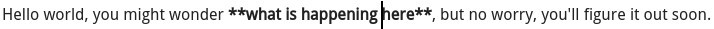
\includegraphics[scale=0.65]{gallery/style_example.jpg}
    \caption[nom dans le sommaire]{Syntaxe Markdown apparente}
    \label{fig:gallery3}
\end{figure}

On constate que le style est appliqué mais que les balises sont encore visibles. Comme indiqué dans le cahier des charges, l'une de mes tâches a été de faire en sorte de cacher la syntaxe.

\subsubsection{Premières approches}
\paragraph{Une approche à la main}
Il s'agissait de la première issue que j'avais à faire. Dans un premier temps, j'ai essayé de résoudre le problème avec "les moyens du bord".
\paragraph{}
Dans mon analyse de la situation, j'ai remarqué que l'utilisation de la syntaxe Markdown au sein de l'éditeur modifiait le DOM \cite{dom}. Le DOM est une interface de programmation qui, entre autres, organise le contenu d'une page HTML en une structure d'arbre qu'il est possible de parcourir et modifier. Si on reprend l'exemple de l'image ci-dessus, on obtient ce DOM, en Figure \ref{fig:gallery4}
\begin{figure}[H]
    \centering
    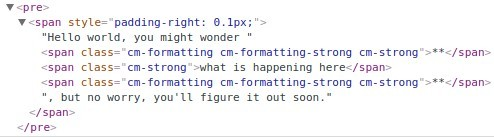
\includegraphics[scale=0.95]{gallery/modified_dom.jpg}
    \caption[nom dans le sommaire]{DOM modifié}
    \label{fig:gallery4}
\end{figure}
\paragraph{}
De ce fait, je pensais faire une recherche des noeuds du DOM dont les classes contiendraient des éléments en rapport avec le style CSS apporté par Markdown. Une fois ce style récupéré il aurait fallu l'appliquer uniquement au "what is happening here". Pour faire disparaître les balises sans pour autant les perdre, j'aurai essayé d'appliquer l'attribut CSS visibility en le mettant à "hidden" aux deux spans contenant les balises.
\paragraph{}
Cependant, cette solution paraissait trop lourde car elle nécessitait un parcours constant du document. De plus, si une personne avait été en train d'écrire, l'édition en aurait été gênée.

\paragraph{}
Mon maître de stage m'a alors suggéré de rechercher des API développées en ce sens à intégrer dans notre projet. Mais aucune n'a montré de résultats concluants.

\subsubsection{HyperMD}
\paragraph{}
Après plusieurs essais avec différentes API, mon maître de stage m'a dirigée vers HyperMD \cite{hypermd}, projet datant de Janvier 2017, et dont la démo \cite{demo} paraissait remplir les objectifs de cette première issue et plus.
\paragraph{}
Après avoir installé HyperMD dans notre projet, nous avons constaté qu'en plus de cacher la syntaxe, les liens étaient stylisés, les images étaient prises en compte, ainsi que les formules mathématiques, grâce à MathJax \cite{mathjax}.
\paragraph{}
MathJax est une librairie open-source, qui, à partir d'une formule respectant une syntaxe particulière, permet de générer un rendu mathématique. HyperMD utilise cette librairie de la manière suivante : il faut encadrer la formule de "\$" ou de "\$\$". Une fois que l'on a fini d'écrire la formule, celle-ci est interprétée. Les dollars disparaissent, et le texte est remplacé par un élément MathJax appelé "jax" qui affiche le rendu stylisé de la formule. Si on clique sur la formule, le jax disparaît, on repasse à une édition de la formule avec les dollars. Lors des premiers tests d'utilisation d'HyperMD, un dysfonctionnement de MathJax m'est apparu : si un collaborateur A modifie une formule, le collaborateur B ne voit pas de modifications de son côté. Cependant s'il clique sur la formule, la formule qui s'affiche en mode édition (avec les dollars) se trouve être la formule écrite par A. Quand il quitte le mode d'édition, MathJax refait le rendu, et B a le même rendu que chez A. Comme il est primordial que dans un contexte collaboratif chaque utilisateur ait la même version du document, j'ai pris l'initiative de créer une issue GitHub décrivant le problème, en y ajoutant le label 'bug'.
\paragraph{}
J'ai aussi pris l'initiative de créer une issue pour créer une cheat-sheet pour MathJax, à l'instar de Markdown, afin d'améliorer l'expérience utilisateur.\\

\newpage
\subsection{Modifier le style}
Afin d'ajouter du style à un texte, il existe un autre moyen que de simplement écrire la syntaxe Markdown à la main. Dans cette partie, nous verrons deux de ces moyens : les raccourcis clavier et les barres d'outils.

\subsubsection{Ajout de raccourcis clavier}
\paragraph{}
Un raccourci clavier est une combinaison de touches permettant d'effectuer une action. A chaque raccourci est associé une action unique. Un raccourci très connu : Ctrl+Z, permet d'annuler la dernière modification effectuée. Dans un éditeur de texte, certains raccourcis ne fonctionnent que si du texte est sélectionné.
\paragraph{}
Les éléments de style pour lesquels il semblait le plus pertinent de créer un raccourci clavier étaient : le gras, l'italique, le fait de rayer un texte et la création d'un lien. Il a ensuite fallu chercher quel est le meilleur raccourci pour ces éléments. Par meilleur, il faut entendre : utilisé dans un maximum d'éditeurs, facile à réaliser et facile à retenir.
\paragraph{}
J'ai jugé qu'il était plus adéquat qu'un raccourci modifie le texte sélectionné plutôt que le DOM. Ainsi, HyperMD n'aurait plus qu'à interpréter les changements effectués.
\paragraph{}
J'ai ensuite créé deux fonctions. La première gère le gras, l'italique et le rayage, la deuxième, les liens.

\paragraph{Gras, italique, rayé}
Pour ces raccourcis j'ai donc associé une liste d'expressions régulières. On utilise une liste car il existe plusieurs syntaxes pour le même style. Par exemple, on peut écrire \_\_exemple\_\_ ou **exemple** pour appliquer du gras.
\paragraph{}
On parcourt la liste d'expressions régulières pour voir si le texte sélectionné contient déjà le style qu'on essaye de lui appliquer.
\begin{itemize}
    \item Si le style n'est pas détecté, on lui applique le style associé au raccourci clavier en ajoutant la syntaxe de part et d'autre de la sélection.
    \item Si le style est détecté, on enlève la syntaxe associée au raccourci clavier. Pour ce faire, on parcourt la sélection des extrémités vers le centre pour enlever la syntaxe correspondante. Juste enlever les extrémités n'aurait pas suffit car il est possible que d'autres styles (et donc d'autres éléments de syntaxes) soient appliqués au texte.
\end{itemize}

\paragraph{Liens}
Un lien en syntaxe Markdown s'écrit de la manière suivante : [texte du lien](url). J'ai pris l'initiative que la partie URL de cette syntaxe soit sélectionnée. Ainsi, l'utilisateur n'a plus qu'à compléter la syntaxe avec l'URL de son choix. J'ai aussi pris en compte le fait que l'utilisateur puisse faire une sélection ne correspondant qu'à une partie de la syntaxe seulement. Le principe algorithmique est le suivant :
\begin{itemize}
    \item Si la sélection "matche" très exactement l'expression régulière, alors on sélectionne la partie URL.
    \item Sinon, on parcourt la sélection.
        \begin{itemize}
            \item Si on a détecté le style CSS associé aux liens (information récupérée grâce au DOM), on continue de parcourir jusqu'à repérer l'expression "(url)" pour pouvoir ensuite la sélectionner.
            \item Sinon le lien n'existe pas, il faut le créer.
        \end{itemize}
\end{itemize}

\paragraph{Limites}
Pour chacun de ces deux cas, une limite est apparue.
\begin{itemize}
    \item L'utilisateur peut faire une sélection grâce à un double clic.  Il se trouve que si l'utilisateur double clique \_\_exemple\_\_, l'entièreté du texte sera sélectionnée, alors que pour **exemple**, seul "exemple" sera sélectionné. Ainsi, si on est dans le cas **exemple** et qu'on utilise le raccourci clavier associé au gras, on ne va pas enlever le gras mais en rajouter. On va alors avoir ****exemple**** avec "**exemple**" en gras. Pour réduire la probabilité que ce cas arrive, les raccourcis claviers associés au gras et à l'italique ont été paramétrés pour utiliser les tirets plutôt que les astérisques.
    \item Il existe un cas pour lequel l'utilisation du raccourci pour les liens n'a pas le comportement attendu. Si on reprend [texte du lien](url), il s'avère que la partie "rl)" ne comporte pas le style CSS associé aux liens. Ainsi, si l'utilisateur sélectionne uniquement cette partie du lien, il va être considéré que la sélection n'est pas un lien, donc un nouveau lien va être créé, au lieu que l'URL soit sélectionnée. On va donc avoir [texte du lien](u[texte du lien](url)rl).
\end{itemize}

\subsubsection{Création d'une barre d'outils}
\paragraph{}
Une nouvelle fonctionnalité de MUTE est l'ajout d'une barre d'outils. Elle sert à ajouter du style (gras, italique, rayé) mais aussi à créer les liens, les citations, les listes et à sélectionner la taille du texte en vue de créer un titre grâce à des boutons ou des menus déroulants. Il a été souhaité qu'elle apparaisse juste au dessus d'une sélection quand une sélection de texte est faite, et disparaisse quand la sélection disparaît. Pour plus d'esthétique, j'ai fait en sorte que le milieu de la barre d'outils corresponde au milieu de la sélection. Cette barre d'outil a été désactivée pour les supports mobile car elle n'est pas bien adaptée à ce genre de support. Il est prévu qu'une barre d'outils similaire soit développée pour apparaître au bas de l'écran, de manière fixe, sur support mobile.
\paragraph{Le composant barre d'outils}
N'ayant trouvé aucune API open-source correspondant aux besoins, il a fallu créer un composant Angular pour intégrer cette barre d'outils. Pour ce faire, j'ai pris connaissance de l'existance de Material Angular \cite{tabs}. Il s'agit de composants Angular représentant des éléments d'interface comme des boutons, des menus déroulants, etc. La barre d'outils est composée de cinq "toggle buttons" et de deux menus déroulants. Le "toggle button" est un bouton à deux états : actif (quand on a cliqué dessus), inactif (après un deuxième clic).
\paragraph{}
Pour qu'un élément d'interface ne soit pas dérangeant, soit intuitif et donne envie d'être utilisé, il m'a été conseillé de lire les directives Angular sur les éléments d'interface REFERENCE. Elles énoncent des principes à respecter et dénoncent les faux pas à ne pas commettre, que ce soit pour la charte des couleurs, la disposition d'un élément ou la manière dont ce dernier doit se déplacer dans l'interface. Ainsi, la barre d'outil est dans les tons orangés, couleur secondaire de la charte des couleurs de MUTE et qui est censée indiquer à l'utilisateur que ces éléments d'interface sont à l'origine d'actions. De même, l'apparition et la disparition de la barre d'outils ont été configurées.
\paragraph{}
En Figure \ref{fig:gallery5}, un aperçu de cette barre d'outils. % \autoref{fig:gallery4} ou \ref{fig:gallery4} >> FIGURE N°figure ou N°figure
\begin{figure}[H]
    \centering
    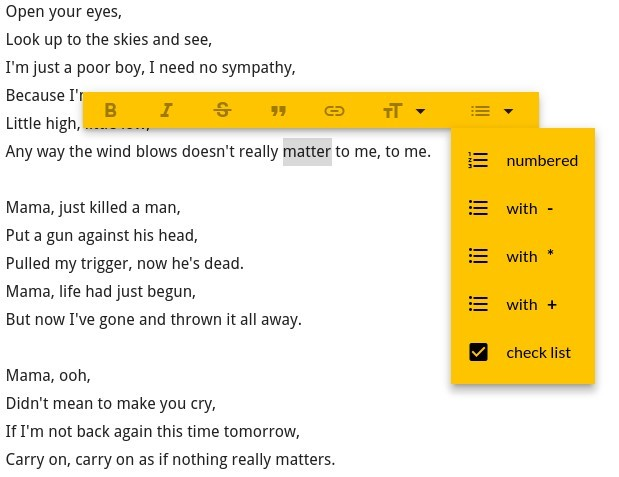
\includegraphics[scale=0.8]{gallery/toolbar.jpg}
    \caption[nom dans le sommaire]{Barre d'outils}
    \label{fig:gallery5}
\end{figure}

\paragraph{Limites}
Une première limite réside en la manière dont sont développés les "toggle buttons" de Material Angular. Il existe un scénario où l'activation de ces boutons se désynchronise d'avec la situation actuelle. Mettons que l'on décide de sélectionner un mot et de le mettre en gras grâce au raccourci clavier. J'ai fait en sorte d'analyser et de récupérer quels styles sont présents dans une sélection, afin qu'à l'apparition de la barre d'outils, les "toggles buttons" soient activés ou non pour le(s) style(s) qui correspond(ent). Une fois le gras appliqué avec le raccourci clavier, le bouton correspondant au gras est dans l'état activé. Si cependant on souhaite retirer le gras grâce au bouton, le gras est bel et bien retiré mais le bouton reste néanmoins dans l'état activé.
\paragraph{}
Une deuxième limite réside en la manière dont CodeMirror gère les copier/coller. Pour CodeMirror, une ligne est représentée par une balise "pre" dans le DOM, caractésirée par une classe "CodeMirrorline". A chaque création de ligne par la touche "Entrée" une nouvelle ligne est créée et dans l'interface et dans le DOM. Mais, si la ligne est créée car la ligne précédente est remplie, CodeMirror ne considère pas ça comme une nouvelle ligne. Ainsi, si on décide de coller un texte de plusieurs lignes dans l'éditeur, il nous apparaît comme un paragraphe de plusieurs lignes. Mais, dans le DOM, on trouve que le texte entier est stocké dans une seule balise "pre". Cela implique que, peu importe où la sélection sera faite dans le paragraphe, la barre d'outils apparaîtra uniquement au dessus de la première ligne du paragraphe.

\newpage
\subsection{Adaptation des appels à MathJax}
MathJax est une librairie offrant une grande diversité de symboles mathématiques qui correspond parfaitement au besoin décrit dans le cahier des charges. Cependant, j'ai relevé un "bug" dans le fonctionnement de cette librairie. Résoudre ce bug ne faisait pas partie de mes issues, mais j'ai pris l'initiative d'essayer de le résoudre. Cependant, la multitude de scénarios possible dans un contexte temps-réel collaboratif fait que j'ai dû me pencher sur le problème qui va suivre à plusieurs reprises car je n'ai pas pu penser à toutes les configurations d'utilisation de ces formules au sein d'un document. Il est d'ailleurs certains que des cas limites ne soient pas encore traités.

\subsubsection{Analyse de la situation}
\paragraph{}
Lors de l'intégration d'HyperMD au projet, j'ai remarqué que si un collaborateur A décidait de modifier une formule, un collaborateur B ne verrait le changement que s'il mettait le focus sur cette formule. Même si cela ne reste qu'un bug d'affichage ne causant pas de divergences \footnote{On parle de divergence quand, pour un même document, les collaborateurs de ce document n'en ont pas la même version à un instant t.}, j'ai proposé à mon maître de stage d'essayer de le corriger avant de m'occuper des cheat-sheets.
\paragraph{}
Dans un premier temps, j'ai essayé de comprendre comment il était possible que l'éditeur du collaborateur B arrive néanmoins à mettre à jour la formule correctement. Il aurait été plus logique qu'au moment de focus ladite formule rien ne se passe de son côté. J'en ai conclu que la syntaxe de la formule mise à jour était donc bien transmise aux collaborateurs.
\paragraph{}
J'ai pensé que l'information pouvait être stockée dans le DOM. Mais je n'ai constaté aucun changement dans le DOM.
\paragraph{}
Pour mieux comprendre comment HyperMD fait appel à MathJax j'ai étudié le code source. Quand une expression du type "\$ ... \$" ou "\$\$ ... \$\$" est détectée, HyperMD créé une marque. Au sens de CodeMirror, une marque est ce qui est utilisé pour "marquer" une partie d'un texte en lui attribuant une classe CSS spécifique. Au moment de créer cette marque, il est possible de spécifier des options. Entre autres, HyperMD décide que l'élément DOM correspondant à cette zone de texte doit être remplacé par un élément span contenant un élément script.
Or, grâce à l'élément script, MathJax est en mesure de générer un rendu. Ce rendu est nommé dans la documentation MathJax "jax".
\paragraph{}
En consultant la documentation de CodeMirror, j'ai constaté qu'il était possible d'avoir accès à l'ensemble des marques. C'est dans cette liste que j'ai retrouvé la syntaxe de la nouvelle formule changée par A (cf en Annexe). En mettant le focus sur la formule, le jax est retiré et la marqué est cassée : on retourne à un aspect d'édition de type "\$ ... \$". Or, comme la marque a été modifiée par A et transmise à B, le contenu de "\$ ... \$" affiché chez B sera bien ce qui se trouve chez A. Une fois que le focus est enlevé, la marque est recréée, MathJax est appelé, et le jax est donc mis à jour. J'en conclus donc qu'il faut forcer MathJax à reprocéder au rendu des formules.\\

\subsubsection{Un premier correctif}
\paragraph{}
Dans un premier temps j'ai procédé comme suit : on récupère les marques et on récupère les jax. On parcourt ces deux listes en parallèle. On récupère le texte contenue dans la marque. A l'aide d'une expression régulière on récupère la formule. On demande à MathJax de s'exécuter avec la nouvelle formule sur la jax correspondante.
\paragraph{}
HyperMD utilisant le même système de marques pour les liens et les images, il ne faut travailler que sur les marques dédiées aux maths. La distinction s'est facilement faite car chacune avait un nom de classe différent.\\
Pour simuler le fait que les rendus soient sensibles à la modification en temps-réel, j'ai utilisé une fonction JavaScript permettant d'exécuter du code selon un intervalle de temps. Je l'ai programmé à cent millisecondes dans un premier temps. Cela ne causait aucun ralentissement dans l'utilisation de l'éditeur.\\

\subsubsection{Extraire les formules}
\paragraph{}
Au hasard de l'utilisation de l'éditeur pendant que je travaillais sur une autre issue, j'ai constaté une anomalie lorsque, sur une ligne, une formule est accompagné d'autres éléments (texte ou autre) :

\begin{figure}[H]
    \centering
    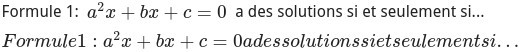
\includegraphics[scale=0.9]{gallery/whole_line.jpg}
    \caption[nom dans le sommaire]{Anomalie de rendu}
    \label{fig:gallery6}
\end{figure}

\paragraph{}
Il semble que MathJax essaye de faire un rendu de tout le texte contenu dans la ligne au lieu de simplement la formule. En regardant de plus près le contenu de la marque il s'avère qu'elle prenait effectivement toute le texte de la ligne en considération.
\paragraph{}
Pour pallier ce problème j'ai donc créé une fonction pour récupérer dans une marque les éléments du texte répondant aux expressions "\$ ... \$" ou "\$\$ ... \$\$". Ainsi, on passe à MathJax la formule au lieu du texte contenu dans la marque.
\paragraph{}
Pour le cas où l'utilisateur soit en train d'ajouter une formule à une ligne en contenant déjà une (imaginer que le texte est "\$ formule 1 \$ \$"), cet algorithme considère que les deux derniers dollars constituent une formule. Cela entraîne des problèmes de rendus qui sont très perturbants pour l'utilisateur en train rédiger. Pour pallier ce problème j'ai donc empêché le rafraîchissement d'une ligne contenant un nombre impair de \$.\\

\subsubsection{Doublons de marques : décalage des rendus}
\paragraph{}
Encore pendant que je travaillais sur une autre issue, j'ai remarqué un décalage dans les rendus MathJax. Par exemple : si sur la ligne 1 se trouvent les formules A et B, sur la ligne 2 la formule C et que l'utilisateur focus la formule B, alors sur la ligne 2 on verra s'afficher le rendu de la formule B. Ce décalage n'est pas transmis aux autres collaborateurs. L'illustration de cette situation est dépeinte dans les Figures \ref{fig:gallery7} et \ref{fig:gallery8}
\begin{figure}[H]
  \begin{minipage}[c]{.46\linewidth}
    \centering
    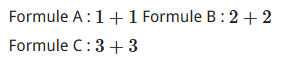
\includegraphics[scale=0.75]{gallery/doublon1.png}
    \caption {\label{fig:gallery7}Situation initiale}
  \end{minipage}
  \hfill
  \begin{minipage}[c]{.46\linewidth}
    \centering
    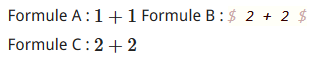
\includegraphics[scale=0.75]{gallery/doublon2.png}
    \caption {\label{fig:gallery8}Décalage du rendu}
  \end{minipage}
\end{figure}
\paragraph{}
Il s'avère que si sur une ligne il y a deux formules, chacune de ces formules va générer une marque. On aura donc deux marques aux contenus identiques. Ainsi, quand la formule B est 'cassée', la marque de la formule A subsiste. Comme on extrait les formules depuis les marques, et comme on itère sur les marques et les jaxs en parallèle, on applique donc à la formule C le rendu de la formule B.
\paragraph{}
Pour pallier ceci j'ai repensé mon code pour pouvoir isoler la ligne contenant une formule en train d'être éditée pour pouvoir toujours garder synchronisés la liste des marques et la liste des jaxs. Toujours en itérant sur les marques, on compte le nombre de formules qu'elle contient :\\
\begin{itemize}
    \item S'il est égal à un, nous sommes dans un cas disons classique, et nous allons juste faire le rendu. Pour être sûr de mettre à jour la bonne jax par rapport à la liste des marques, on met en place un compteur symbolisant index de la prochaine jax à mettre à jour.
    \item S'il y a plusieurs formules dans cette marque, on stocke ce nombre et on passe à la marque suivante :\\
    \begin{itemize}
        \item Si la marque est différente et qu'on n'a pas passé autant de marques que le nombre de formules détectées, c'est que l'une d'elle est en édition. On ne met rien à jour et on augmente le compteur de la prochaine jax à mettre à jour.
        \item Si la marque est identique mais qu'on n'a pas passé autant de marques que de formules détectées alors on ne fait rien et on passe à la marque suivante.
        \item Si la marque est identique et qu'on a passé le bon nombre de marques alors aucune des formules n'est en train d'être éditée et on peut alors faire un rendu.
    \end{itemize}
\end{itemize}

\subsubsection{Limites}
\paragraph{}
Cette problématique à elle seule aurait dû constituer une issue plus importante que simplement une issue avec le label 'bug'. Cependant je devais aussi avancer sur d'autres fonctionnalités donc mon travail n'est pas aussi complet que ce que je l'aurai souhaité. Par exemple, la solution mise en place actuellement bloque le rendu des jaxs des lignes contenant un nombre impair de '\$'. Or il est possible que ce cas subvienne. Néanmoins, la mise à jour des formules est toujours possible si on focus la formule.
\paragraph{}
L'utilisation de MathJax a montré quelques difficultés lors d'un test réalisé avec neuf navigateurs. Des fois les formules disparaissaient complètement. Il est difficile de reproduire les scénarios où MathJax a dysfonctionné.
\paragraph{}
Avec un intervalle de cent millisecondes, il arrivait des fois que toutes les formules s'affichent en deux fois si on cassait/reformait les marques trop vite. Ce bug ne touche pas aux marques et disparaissait très rapidement. Pour régler le problème, l'intervalle est de maintenant trois secondes. Si cela sacrifie un peu le caractère 'temps-réel' cela offrira peut-être une meilleure stabilité au fonctionnement de MathJax en collaboration.

\newpage
\subsection{Création d'antisèches}
\paragraph{}
Afin d'améliorer l'expérience des utilisateurs de MUTE, deux issues ont été créées pour ajouter des cheat-sheets à l'éditeur, littéralement des antisèches. Ces antisèches contiendraient des rappels de syntaxe pour Markdown et MathJax. Nous avons décidé avec mon maître de stage que ces éléments seraient incrustés à droite du document, au même niveau que les informations le concernant (localisation du stockage et collaborateurs), afin que l'utilisateur puisse les avoir à portée tout en gardant accès à l'éditeur. Il m'a été suggéré de réfléchir à une solution à base d'onglets à intégrer au niveau du composant nommé très justement "right-side".
\paragraph{}
Via mes recherches pour la barre d'outils, je me suis souvenue qu'Angular Material proposait un module Tabs (onglets). J'ai donc immédiatement travaillé sur cette solution. J'avais alors deux manières d'organiser les informations : soit avoir trois onglets (Details, Markdown, MathJax), soit avoir deux onglets (Details, Cheat-sheets) avec dans Cheat-sheets deux onglets (Markdown et MathJax). J'ai opté pour la deuxième solution, car trois onglets prenaient trop de place, le nom des onglets était tronqué. De plus cela fait plus de sens de stocker toutes les cheat-sheets dans un même onglet.\\

\subsubsection{Markdown Cheat-sheet}
\paragraph{}
Pour le contenu, et après avoir regardé des équivalents sur d'autres éditeurs, j'ai opté pour une disposition sur deux colonnes avec à gauche le rendu, à droite la syntaxe associée. L'idée que j'avais était d'avoir un rendu intuitif et raccord avec le reste de l'interface et les guidelines Angular.
\paragraph{}
J'ai tout d'abord essayé de travailler avec les tables HTML, mais le rendu était peu satisfaisant. Le fait de voir un tableau à cet endroit paraissait trop scolaire, le rendu était trop chargé.\\
J'ai englobé le contenu dans un card, un autre composant Angular. Pour comprendre à quoi cela correspond, la zone d'édition du document, ressemblant beaucoup à feuille blanche, est un card. Cela m'a donné l'idée qu'il serait intéressant pour l'utilisateur de voir ce que le rendu donne réellement sur le document. Ainsi, et pour donner de la structure à l'antisèche, j'ai mis le card en gris clair, puis y ait inséré six autres cards, eux en blanc. Chacun de ses cards représentera les catégories suivantes : les headers, les styles, les listes, les images, les liens et le code informatique. J'ai créé ces catégories en m'inspirant de cette cheat-sheet Markdown \cite{mdcheat}. Précédant chacun de ces cards, un titre en gris foncé, taille h2 permet de nommer chacune de ces catégories et sert de séparateur naturel entre chacun des cards.
\paragraph{}
Afin que les rendus soient fidèles à ce que génère HyperMD, j'ai eu l'idée d'importer la feuille CSS liée à HyperMD dans la feuille CSS du right-side. Ainsi, pour chaque texte auquel je voudrais appliquer le rendu HyperMD je n'aurai qu'à appeler la classe correspondante. Mais le style ne s'appliquait pas. Après plusieurs essais, j'ai décidé recréer des classes dans la feuille de style de right-side pour reproduire le rendu HyperMD.
Cette solution a marché mais cela a produit une duplication de code, il y a certainement moyen de faire autrement.
\paragraph{}
Après présentation à mon maître de stage, celui ci m'a suggéré que le fond gris clair soit de même couleur que l'arrière plan de l'application. Ainsi, les cards ressortent vraiment, sont à la même élévation que la zone d'édition et donnent un effet "post-it" qui est, je pense, vraiment parlant pour l'idée de mémo. L'utilisateur a donc une réelle idée du rendu que peut avoir ces différentes syntaxes.
\paragraph{}
Enfin, mon maître de stage a également suggéré que la cheat-sheet ait son propre composant Angular, sous-composant de right-side.\\

\subsubsection{MathJax Cheat-sheet}
\paragraph{}
Pour cette antisèche, je suis partie sur le même concept d'apparence et de structuration.
\paragraph{}
Dans un premier temps, mon maître de stage et moi-même désirions que les rendus des formules soient générés par MathJax. MathJax étant utilisé uniquement par HyperMD, je n'avais jamais eu besoin de l'importer au sein de notre projet. Cette tâche seule s'est étalée sur trois jours. Pour ne pas pas perdre trop de temps, en parallèle, je commençais de mettre en place le composant qui allait contenir l'antisèche. Finalement, après que mon maître de stage soit venu m'aider à mettre en place MathJax, nous avons constaté qu'une particularité de MathJax était bloquante : en effet, MathJax charge les formules globalement, sur l'ensemble de l'interface. Plus précisément : la liste de 'jax' mentionnée en 3.6 est unique à l'application. Ainsi, les rendus se retrouvaient décalés : la première formule dans l'éditeur avait son rendu dans l'antisèche, et toutes les autres formules se trouvaient décalée d'un cran.
\paragraph{}
Nous avons donc conclu qu'il serait plus simple que les rendus dans l'antisèche soient des images provenant d'impressions d'écrans. L'avantage à cela est que le rendu correspondra tout à fait à ce que MathJax produit dans l'éditeur, de plus, cela fait moins de formules à charger lors de l'affichage de l'antisèche.\\

\subsubsection{Inconvénients}
\paragraph{}
HyperMD prévoit que tout texte collé dans l'éditeur à partir du presse-papier soit automatiquement échappé. Par exemple, *Hello world!* devient \textbackslash*Hello world!\textbackslash*. Il en va de même si l'utilisateur choisit de copier/coller la syntaxe d'un élément l'intéressant de l'antisèche vers l'éditeur. En soit ce n'est pas vraiment une mauvaise chose, car l'utilisateur pourra effectuer des manipulations avant d'enlever les caractères d'échappement et que le rendu ne se fasse. De plus les sections copiées ne sont pas très longues. Mais cela nécessite quand même une manipulation supplémentaire. Sans compter que pour des utilisateurs moins au fait de l'utilisation de l'éditeur cela peut poser un problème de compréhension.
\paragraph{}
Un autre inconvénient vient de l'utilisation des Tabs. Dans l'onglet Details se trouve l'affichage des contributeurs du projet. Il se trouve que le contenu de cet onglet refusait de prendre tout l'espace. Ainsi, le contenu était réduit à un très petit espace, qui, par conséquent, générait une barre de défilement, ce qui n'était pas très esthétique. Mon maître de stage a pris en charge la résolution de ce problème. Cela a eu un effet sur les antisèches, qui ne sont plus contenues dans un card gris, mais sont juste disposées sur le fond de l'application. Le résultat reste très sensiblement le même.
\paragraph{}
Le dernier inconvénient vient de la manière dont sont implémentées les Tabs d'Angular Materiel. La première fois que l'on décide de consulter les cheat-sheets, les deux sous-onglets se découvrent et l'on voit par défaut la cheat-sheet Markdown. Or, l'onglet Markdown n'est pas marqué comme étant sélectionné. Le résultat de ce travail est visible Figure \ref{fig:gallery9}.

\begin{figure}[H]
    \centering
    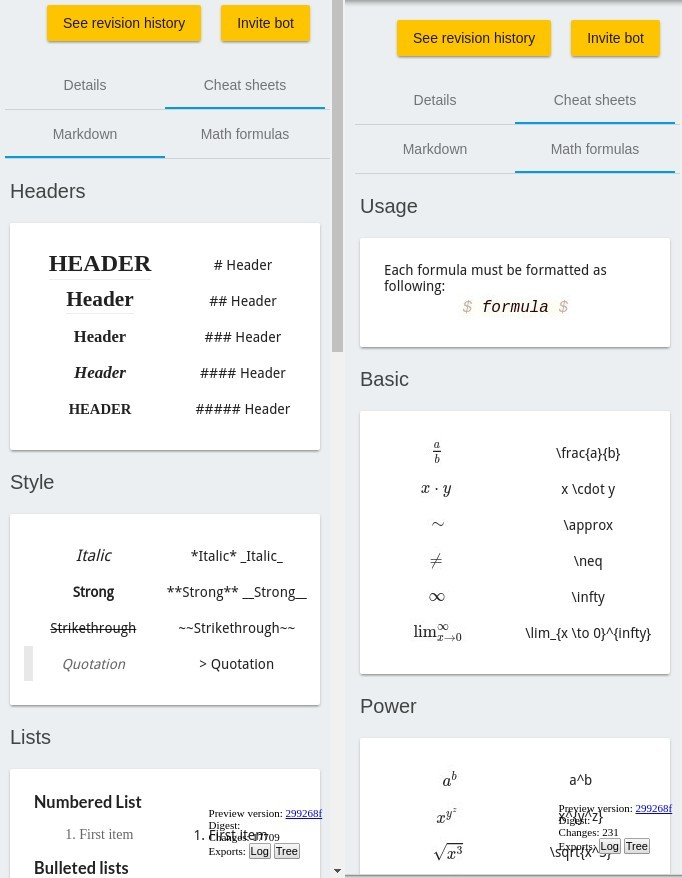
\includegraphics[scale=0.7]{gallery/cheat-sheets.jpg}
    \caption[nom dans le sommaire]{A gauche l'antisèche Markdown, à droite l'antisèche MathJax}
    \label{fig:gallery9}
\end{figure}


\newpage
\subsection{Tests}
\paragraph{}
Au cours du stage, il est arrivé que mon aide soit requise pour des tests. En effet, si l'on peut plus ou moins tester la robustesse de notre développement en ouvrant plusieurs navigateurs à la fois, il est impossible de reproduire l'édition simultanée d'un document par plusieurs collaborateurs. C'est pourquoi mon maître de stage, d'autres collègues, voire même moi-même demandions un coup de main à d'autres. Ces tests permettaient aussi que d'autres mettent en avant des scénarios où le développement de l'un ou de l'autre était incomplet.
\paragraph{}
De plus, chaque compte rendu des réunions hedbomadaires était pris via MUTE. Nous pouvions ainsi tester la dernière démo, ce qui permettait de mettre en avant des oublis, des bugs ou des précisions sur les cas d'utilisations.\\

\newpage
\section{Bilan du stage}
\subsection{Avancement par rapport au cahier des charges prévu}
\paragraph{}
Si on se réfère au cahier des charges, la majorité des tâches a été accomplie. Il faut comprendre que l'on m'a attribués les issues en rapport avec la thématique de mon stage. Il y avait toujours possibilité d'ajouter d'autres tâches en rapport avec mon travail. En somme, il n'y a pas de réelle fin à ce travail. Mon travail a été apprécié dans son ensemble.

\subsection{Retombées}
\paragraph{}
MUTE et donc mon travail sont disponibles sur le serveur de production \footnote{\href{https://www.coedit.re}{https://www.coedit.re}}. L'éditeur sera utilisé chaque semaine lors des réunions hebdomadaires de l'équipe. De plus, l'éditeur sera présenté à l'ECSCW à Sheffield.
\paragraph{}
L'algorithme qui effectue la fusion des collaborations ne travaille qu'avec du texte brut. Ainsi, mon travail a permis de mettre en avant la possibilité de transférer du style et même des formules mathématiques grâce à ce seul algorithme en travaillant avec des API de parsing de texte. Si cela n'avait pas marché, il aurait fallu développer une autre structure pour transférer le style.

\subsection{Développement futur}
\subsubsection{Barre d'outil responsive}
Comme précisé dans la partie correspondante, la barre d'outil n'est pas responsive. Même s'il s'agit d'un détail, il reste toujours très apprécié et est un gage de qualité au sein d'une application.

\subsubsection{Attendre les nouvelles versions de certaines dépendances ?}
Certaines limites de développement évoquées dans ce rapport tiennent dans la manière dont sont développées certaines librairies.

\paragraph{HyperMD}
Le projet HyperMD et MUTE présentaient une issue en commun : la création d'une barre d'outils. Au cours de mon analyse des fonctionnalités proposées par HyperMD j'ai dressé une liste des issues ouvertes sur ce projet et qui peut impacter le nôtre :
\begin{itemize}
    \item interprétation des paragraphes
    \item interprétation des tableaux
\end{itemize}
Après être entré en communication avec le propriétaire de ce projet il s'avère qu'HyperMD n'est pas sa priorité numéro une. Il conviendrait donc de traiter ces cas nous-mêmes.

\paragraph{MathJax}
Une particularité de cette librairie qui la rend unique face aux librairies utilisées dans MUTE est qu'elle est globale à l'application. Il serait préférable qu'on puisse la configurer pour la rendre globale à un document particulier. Depuis 2015, il est possible de voir sur le répertoire GitHub de ce projet qu'une version 3 est en cours de réflexion. Il semble donc qu'il se déroule une certaine période avant d'obtenir quelque chose de plus stable. Il serait peut-être envisageable de trouver une autre librairie qui remplisse les besoins escomptés.

\paragraph{Angular Material}
Au contraire de MathJax, le projet Angular Material semble plus actif. Il est donc très probables que les deux limites énoncées à l'encontre de l'utilisation d'Angular Material soient corrigées prochainement, mais elles représentent très certainement une priorité faible.

\subsubsection{Une nouvelle fonctionnalité : paramètres}
\paragraph{}
A l'issue de ce stage, beaucoup de nouvelles fonctionnalités ont été mises en place. Toujours soucieuse de l'expérience utilisateur, j'ai imaginé qu'il serait intéressant de mettre en place un système de paramétrage de certaines options.
\paragraph{}
Ainsi on pourrait laisser à l'utilisateur le soin de pouvoir activer/désactiver la barre d'outils, et les previews MathJax. Mais aussi, quand beaucoup de formules sont chargées au sein d'un même document, si la configuration de l'ordinateur de l'utilisateur met en cause le bon fonctionnement de MUTE, demander à augmenter l'intervalle de rafraîchissement des formules. Dans le même soucis de performances, s'il y a beaucoup de collaborateurs sur le même document, ou tout simplement par confort, animer le curseur d'un collaborateur seulement quand il écrit, voire complètement les désactiver.
\paragraph{}
Pour mettre en place cette fonctionnalité, on pourrait mettre en place un bouton paramètres dans le menu gauche de MUTE. Ce bouton pourrait faire apparaître une boîte de dialogue comportant la liste des différents paramètres cités précédemment. En face de ces éléments, on pourra mettre en place un objet d'Angular Material. Pour les activations/désactivations, des slige toogles \cite{slide}. Pour régler la fréquence des rafraîchissements et la complexité des animations, des sliders \cite{slider}.\\

\subsubsection{Améliorations des appels à MathJax}
\paragraph{}
En attendant une version plus stable de MathJax, et si aucune autre librairie viendrait à se substituer à celle-ci, nous avons discuté avec mon maître de stage de certaines dispositions qui pourraient être mises en place pour limiter son dysfonctionnement.
\paragraph{}
Dans un premier temps, il serait possible de ne plus demander le rendu des formules selon un intervalle de temps mais seulement quand une modification est perçue. S'il m'était possible de pouvoir détecter une modification, je n'ai cependant pas eu l'idée de comment récupérer cette information d'HyperMD et de la transmettre à MUTE.
\paragraph{}
Grâce à l'API Netflux, il est possible d'ajouter au réseau pair-à-pair un "bot". L'idée première de cette fonctionnalité est de permettre à un utilisateur de pouvoir stocker son document sur la base de données OVH (où est hébergé MUTE) en plus de la base de données native du navigateur internet. Ce bot est relié à tous les autres pairs et peut aussi servir à faire des calculs qu'on lui aurait délégué. Ainsi, il serait possible de déléguer le rendu des formules MathJax à ce bot qui n'aurait plus qu'à transmettre le résultat aux autre pairs. Ainsi, les navigateurs pourraient s'affranchir de toutes ces requêtes MathJax.
\paragraph{}
Il en va sans dire que s'il était possible d'associer ces deux dispositions, on obtiendrait une utilisation moins prenante en ressources et certainement plus stable.\\

\newpage
\addcontentsline{toc}{section}{Conclusion}
\section*{Conclusion}
\paragraph{}
L'objectif de ce stage a été d'apporter des fonctionnalités autour de l'ajout de style au sein de MUTE. Grâce à des solutions open-source ou à des directives reproductibles au sein du projet, nous avons vu comment l'éditeur a évolué au cours de ces dix semaines. Nous avons également vu les limites de ces solutions.
\paragraph{}
Après discussion avec mon maître de stage, celui-ci m'a fait prendre conscience que les entreprises développent elles-mêmes les outils qui leur permettent de remplir leurs besoins. Donc, au contraire des entreprises, on réalise que les équipes de recherches, même si elles sont en première ligne dans les avancées technologiques et théoriques, sont aussi les premières à pâtir des limites de ces dernières. En l'occurrence ici, on constate que le développement des solutions que j'ai apportées sont soumises au développement des API, donc au travail de beaucoup de personnes. Certaines d'entre elles développent ces API dans un but de loisir et non professionnel. De plus, mon maître de stage m'a indiqué que le principe d'une équipe de recherche est de montrer qu'il est possible de mettre en place des solutions novatrices. En l'occurrence nous avons montré qu'il est possible d'ajouter la gestion de style, de formules mathématiques et de listes tout en gardant l'algorithme de fusion initial LogootSplit.
\paragraph{}
Le fait de travailler en équipe de recherche m'a fait réaliser deux choses. La première est qu'il est difficile d'atteindre le résultat parfait dans le contexte de la recherche et des projets open-source. J'attends mon expérience en entreprise en troisième année pour confirmer ou infirmer cette impression. La deuxième chose est qu'évoluer dans ce contexte, ou en tout cas dans l'équipe COAST, permet de travailler en toute autonomie. Chaque idée ou piste de recherche de solution est valorisée, ce que je trouve très motivant.

\newpage
\printbibliography[heading=bibintoc,title={Webographie}]

\newpage
\addcontentsline{toc}{section}{Glossaire}
\section*{Glossaire}

\clearpage

\newpage
\addcontentsline{toc}{section}{Annexes}
\section*{Annexes}
\subsection*{Annexe A}
\begin{figure}[H]
\centering
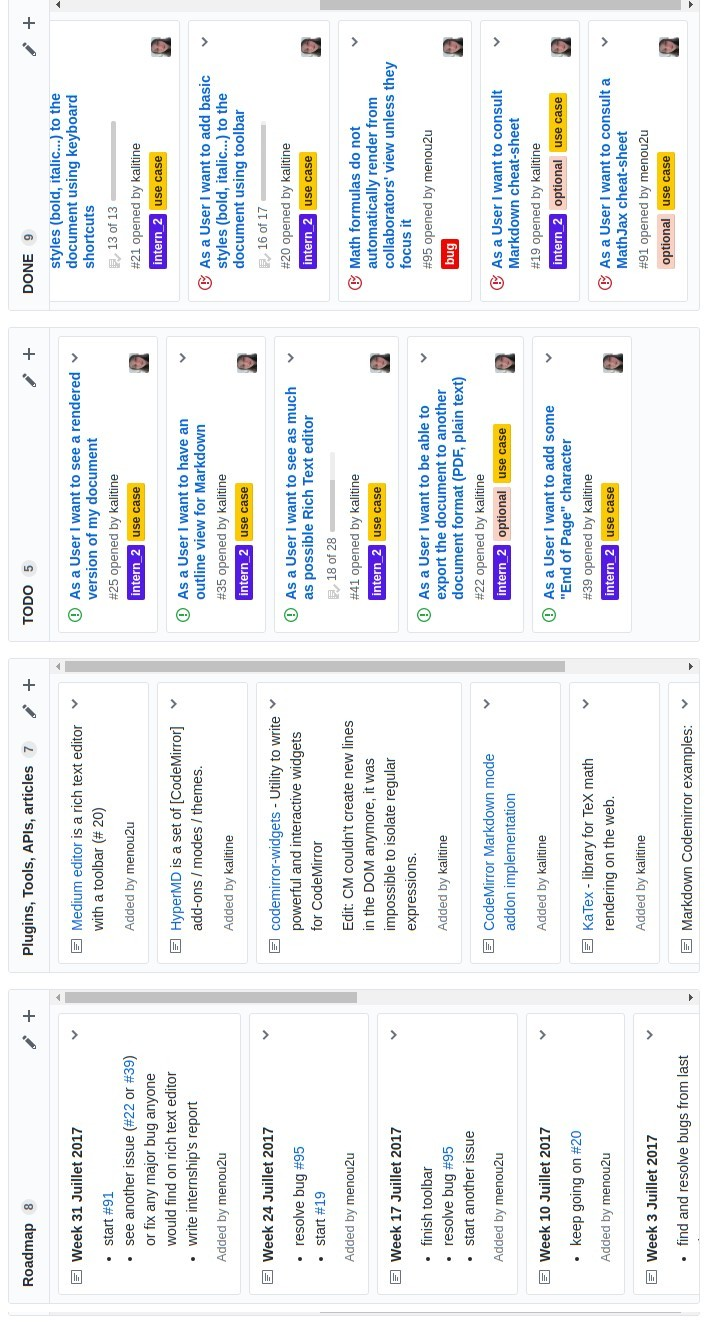
\includegraphics[scale=0.52]{gallery/workboard.jpg}
\caption[nom dans le sommaire]{Workboard du projet Rich Text Editor}
\label{fig:gallery1}
\end{figure}

\newpage
\subsection*{Annexe B}
\begin{figure}[H]
\centering
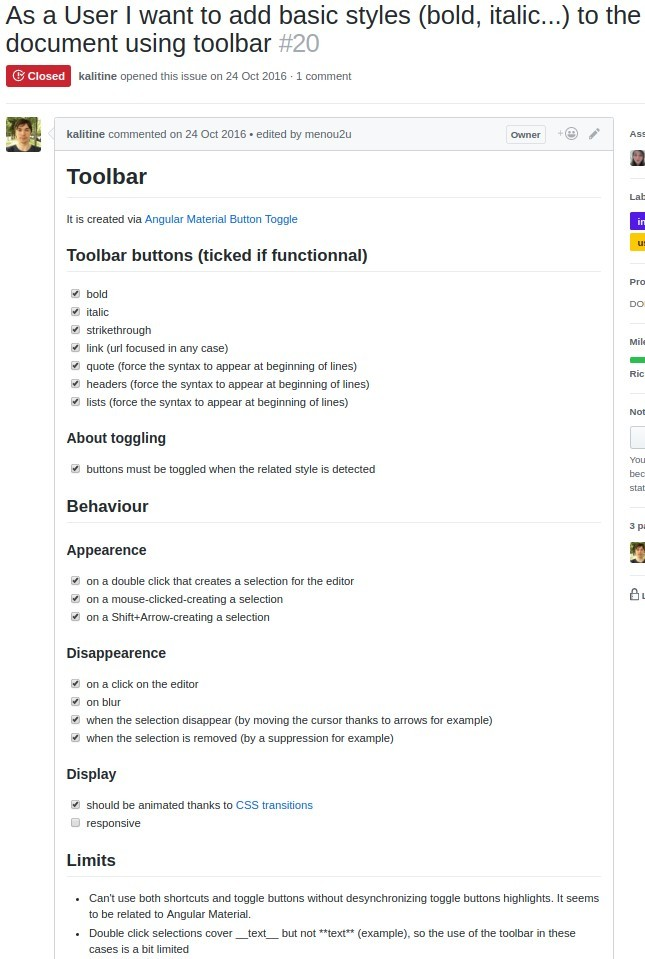
\includegraphics[scale=0.75]{gallery/issue.jpg}
\caption[nom dans le sommaire]{Issue associée à la barre d'outils}
\label{fig:gallery2}
\end{figure}

\newpage
\section*{Mots-clefs :}
\textbf{interopérabilité, collaborative-editing, Angular}

\end{document}